\chapter{基于分布式文件系统GlusterFS的数据迁移研究}

\section{GlusterFS介绍}

GlusterFS\cite{GlusterFS}是一个开源、扩展能力强大的分布式文件系统,其客户端与存储服务器可通过InfiniBand RDMA或者TCP/IP等多种方式连接,并使用统一的命名空间管理数据,可将不同类型的存储服务器整合在同一个命名空间中,从而为各种工作负载和应用场景提供出色的性能。 GlusterFS服务器兼容POSIX标准,支持诸如ext4、XFS等{\color{orange}扩展属性文件系统},可以使用包括网络文件系统(Network File System)和SMB(Server Message BLock)等在内的业界标准访问协议进行访问。GlusterFS专为当前高性能虚拟化云环境而设计,也可用于在并行文件系统之上搭建大规模科学与工程计算文件系统。 

本节将对GlusterFS的架构与原理作简要介绍,并重点分析其数据迁移模块Tiering。
\subsection{整体架构和原理}
%\begin{itemize}
%    \item 全局命名空间。
%    \item 集群存储管理。
%    \item 模块化的层次机构。
%    \item 内置replication and geo-replication特性。
%    \item 自修复功能。
%    \item 高效负载均衡。
%\end{itemize}
\begin{figure}[htp]
\centering
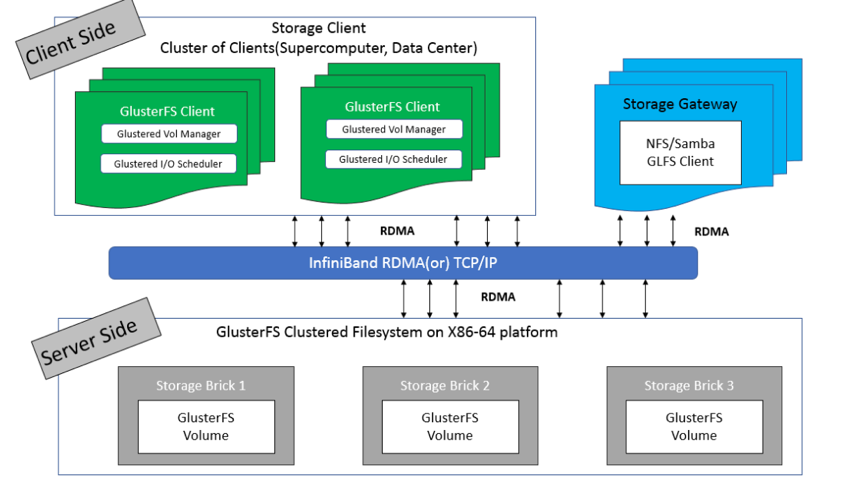
\includegraphics[width=\textwidth]{GlusterFS_Arc}
\caption{GlusterFS整体架构图}
\label{fig:GlusterFS_Arc}
\end{figure}
如图\ref{fig:GlusterFS_Arc}所示,GlusterFS服务端以存储块(Storage Brick)为硬件存储单元,可挂载于磁盘、固态硬盘、内存等多种存储介质。逻辑卷(Volume)是文件系统中的逻辑存储单元,每一个逻辑卷可由一个或者多个存储块构成,绝大多数gluster管理操作是在卷上进行的。GlusterFS根据用户需求能够支持多种逻辑卷,主要包括:

{\color{red}这里itemize的格式有问题}

\begin{itemize}
    \item 分布式卷(Distributed Volume)。文件通过hash算法将数据分布到所有存储服务器上,这种卷是glusterfs的基础和最大特点;其本质功能是扩大的磁盘空间,如果有一个磁盘损坏,其数据也丢失,文件级RAID 0,不具有容错能力。
    \item 复制卷(Replicated Volume)。此类逻辑卷将文件同步复制到多个brick上,文件级RAID 1,具有容错能力,同等硬件条件下写性能下降,但读性能有所提升。
    \item 条带卷(Stripe Volume)。类似RAID0,文件分成数据块以Round Robin方式分布到存储服务器上,并发粒度是数据块,支持超大文件,大文件的读写性能优异。
    \item 复合卷。所谓复合卷主要包括分布式条带卷、分布式复制卷、条带复制卷和分布式条带复制卷等,兼具了基本卷的优点,在实际应用场景下较常见。
\end{itemize}

\begin{figure}[htp]
\centering
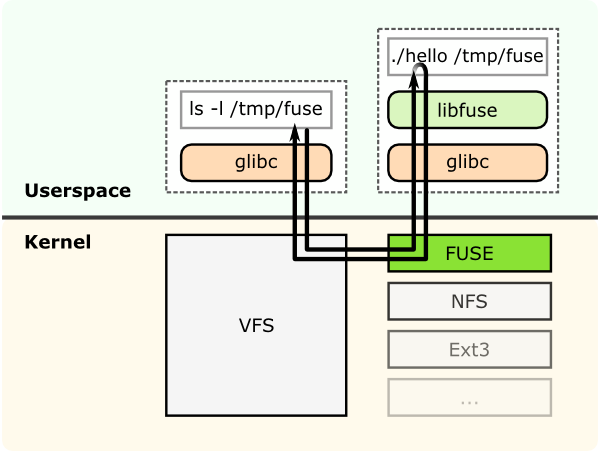
\includegraphics[width=\textwidth]{fuse}
\caption{用户空间文件系统}
\label{fig:fuse}
\end{figure}
GlusterFS是一个用户空间文件系统,采用了FUSE(File System in Userspace){\color{red}(此处应有引用)}作为用户态程序与内核文件系统交互的接口。如图\ref{fig:fuse}所示,

\subsection{层叠式模块设计}
\begin{figure}[htp]
\centering
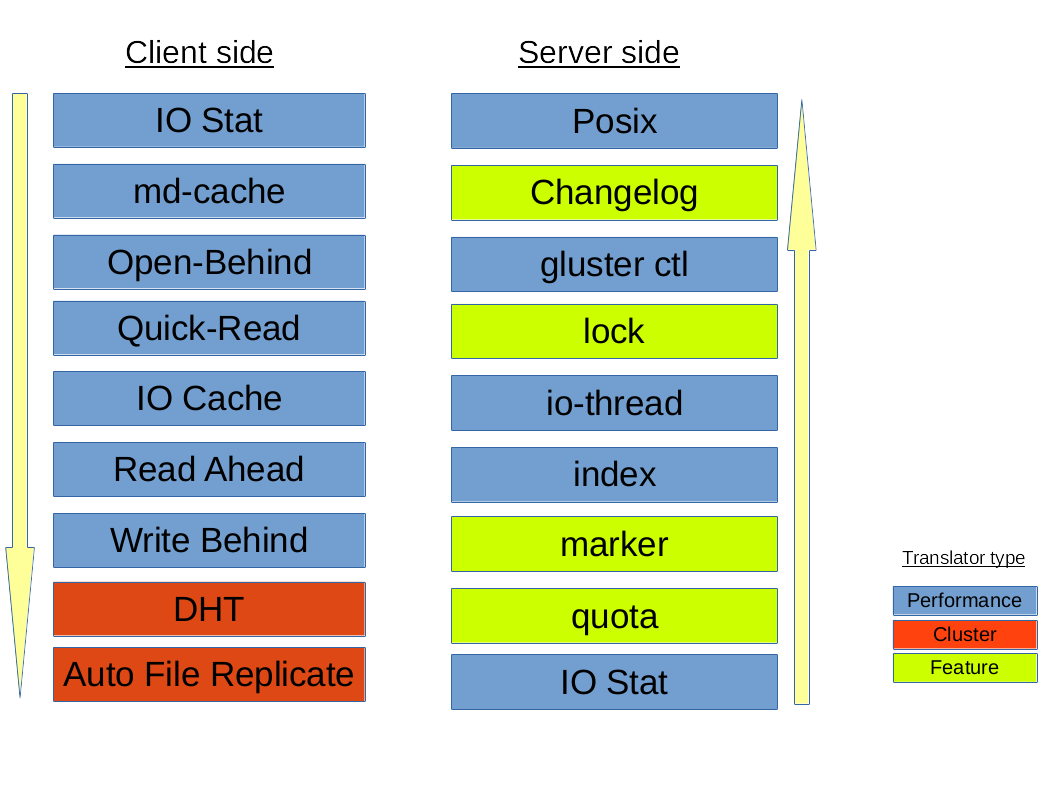
\includegraphics[width=\textwidth]{translators}
\caption{由翻译器(Translators)堆叠组成的堆栈式结构}
\label{fig:translators}
\end{figure}
\section{基于GlusterFS Tiering功能的缓存管理模块设计}
\subsection{Trace 模块}
\subsection{访问模式识别模型建立}
\subsection{运行时缓存管理}


\section{本章小结}